\clearpage
\fancyhead[R]{\small\color{muted}Vulkan · Sponza}
\section{中庭雕塑展}
主相机朝着中庭的长廊。玉绿色的龙占据画面中央，两侧分别放了赤陶色的兔子和赭色的佛像。三件雕塑采用 Stanford 的扫描网格，台座则直接用引擎的立方体。模型尺寸各不相同，摆放时先将它们缩放到想要的高度，再将各自最低的顶点移到台面。这样改龙的大小时，它的脚还能落回原处。

\begin{figure}[H]\centering
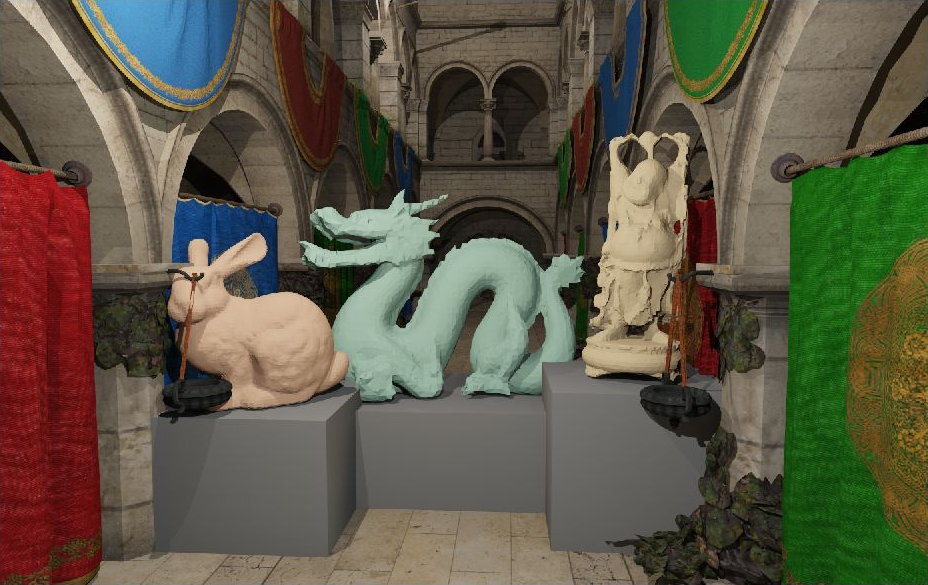
\includegraphics[width=.96\linewidth]{Sponza-Sculpture-Gallery.png}
\caption{RedflagForge 实际 Game 视口。展品的摆放、材质底色、灯光和机位保存在场景文件中。}
\end{figure}

要接着布光，先在主相机视图看一眼龙的轮廓，再回到场景视图选「主灯」。这盏暖色点光源从前侧照向雕塑。另一侧的冷光把龙的头颈从深色布景中分出来。镜头前还有一盏名为「补光灯」的点光源，降低它的强度可以看到龙身凹处的阴影加深。主相机留在原处，在两个视图之间切换，能看清移灯究竟改变了雕塑的哪一面。保留机位，在「实时效果」勾选「对照：只显示直接光」，还可以单独看灯直射到的部分，取消勾选即可看回完整光照。

资源准备好后，在项目面板双击 \path{Sponza-Sculpture-Gallery.redflag}。首次在新机器上打开时，从仓库根目录分别运行 \path{python tests/fetch_sponza.py} 与 \path{python tests/fetch_stanford.py}。原始网格和纹理按各模型的来源及使用条件提供，场景文件只保存对模型的引用。
\par\noindent
\source{https://graphics.stanford.edu/data/3Dscanrep/}{Stanford 扫描模型}
\quad\source{https://github.com/KhronosGroup/glTF-Sample-Assets/tree/main/Models/Sponza}{Khronos · Sponza 模型与许可}
